\documentclass[10pt,a4paper]{report}
\usepackage[utf8]{inputenc}
\usepackage{amsmath}
\usepackage{amsfonts}
\usepackage{amssymb}
\usepackage{graphicx}
\author{Paolo Mazza}
\title{Tree from space colonization}
\begin{document}
Paolo Mazza\qquad \qquad\qquad\qquad\qquad\qquad\qquad1693404\\\\
Trees-generator è un generatore di alberi basato sull'algoritmo di space colonization. E' un'implementazione in C++ del metodo di generazione di alberi illustrato ad alto livello in [RLP07] \footnote{[RLP07] Runions A., Lane B., Prusinkiewicz P.: Modeling Trees with a Space Colonization Algorithm. Eurographics Workshop on Natural Phenomena (2007)}, che esplora un modello basato sulla competizione dei rami per lo spazio per determinare la forma degli alberi.\\\\
Tree-generator riceve in input un'envelope, cioè un modello in formato .obj all'interno del quale l'albero sarà costruito. Il modello seguito si sviluppa intorno alle seguenti funzioni, chiamate nel seguente ordine:
\begin{itemize}
\item \textbf{generate\_attraction\_points} prende in considerazione i punti che formano l'envelope e genera un numero -n (default è 1000) di attraction points, così ottenuti:
\begin{enumerate}
\item sceglie due punti, \emph{f} e \emph{s}, casuali dell'envelope utilizzando le funzioni next\_rand di Yocto GL
\item l'attraction point generato è un punto casuale che giace sull'intervallo "interno" della retta passante per \emph{f} e \emph{s} 
\end{enumerate}
\begin{figure}[h]
\centering
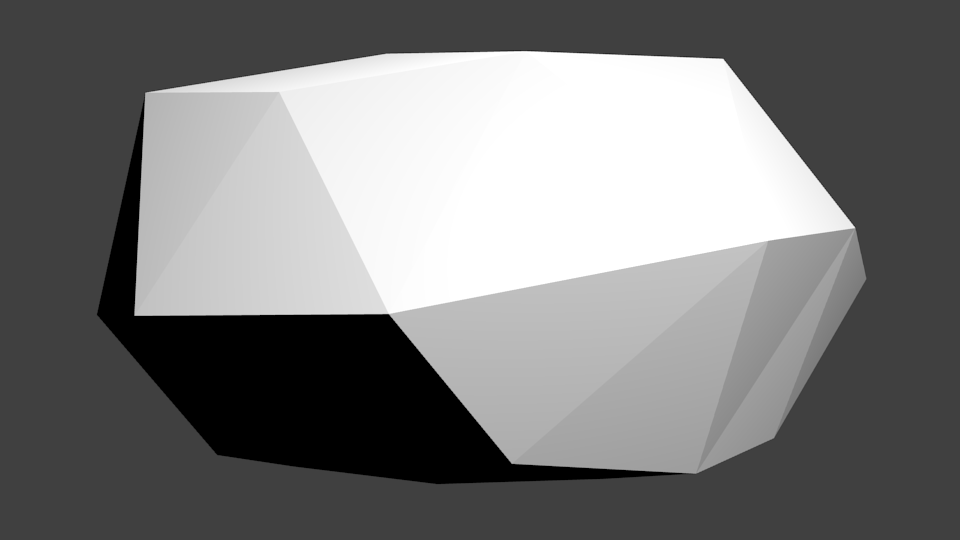
\includegraphics[scale=0.37]{envelope.png}
\caption{Envelope generata usando Blender}
\end{figure}
\begin{figure}[h]
\centering
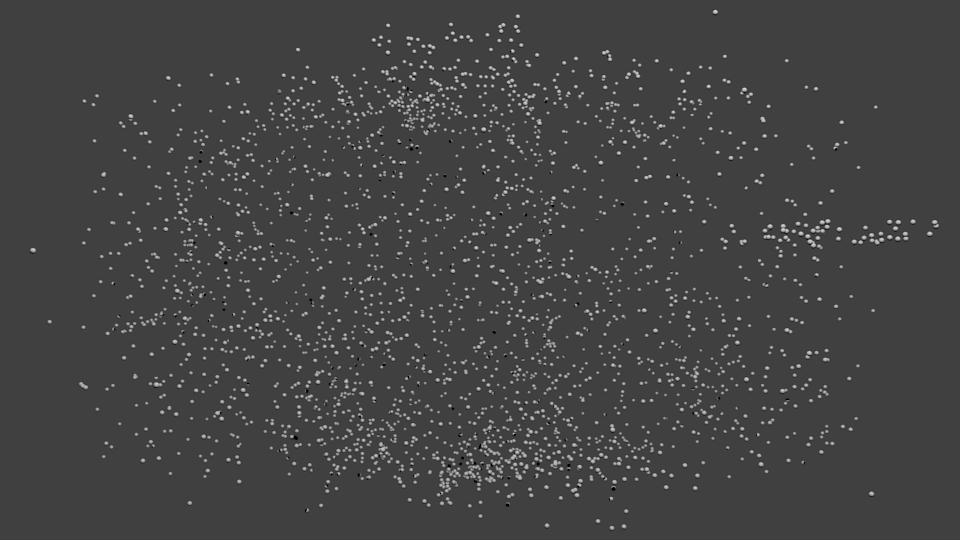
\includegraphics[scale=0.37]{points.png}
\caption{Distribuzione casuale di 3000 attraction points}
\end{figure}
\item \textbf{generate\_nodes} prende in input l'insieme degli attraction points, un base node (la radice dell'albero che verrà generato), la distance of influence (la distanza massima entro la quale un attraction point può influenzare un nodo), la kill distance (se un nodo si trova una distanza minore di questa da uno specifico attraction point, questo viene eliminato e, conseguentemente, non influenzerà i nodi nelle iterazioni successive) e una distance (la distanza tra un nodo e quelli da lui generato), mantenendo durante la procedura quattro vettori: nodes, children (vettore dei figli; un vettore per ogni nodo, contenente gli indici dei figli nel vettore nodes), parents (vettore dei genitori; indice del genitore nel vettore nodes) e nodes\_norm (vettore delle normali; direzione della retta tra nodo padre e nodo figlio).\\\\
Genera iterativamente nuovi nodi partendo dal base node finchè non ci sono nodi influenzati da attraction points.\\ A ogni iterazione:
\begin{itemize}
\item calcola per ogni nodo $v$ l'insieme degli attraction points che lo influenzano $S(v)$ (ogni attraction point influenza il solo nodo a lui più vicino) e la direzione $\vec{n}$ di crescita del nodo  $$ \vec{n}=\sum_{s \in S(\nu)} \frac{s-\nu}{||s-\nu||}$$
\item calcola per ogni nodo influenzato da almeno un attraction point il nuovo nodo $v'$ posizionato a distanza $D$ (dato in input) da $v$ in direzione $\hat{n}$
 $$\hat{n}=\frac{\vec{n}}{||\vec{c}||} \qquad and \qquad v' = v + D\hat{n}$$
\item per ogni nuovo nodo aggiorna il vettore dei genitori, dei figli e delle normali ed elimina gli attraction points che si trovano a distanza minore di kill distance
\end{itemize}
\begin{figure}[h!]
\centering
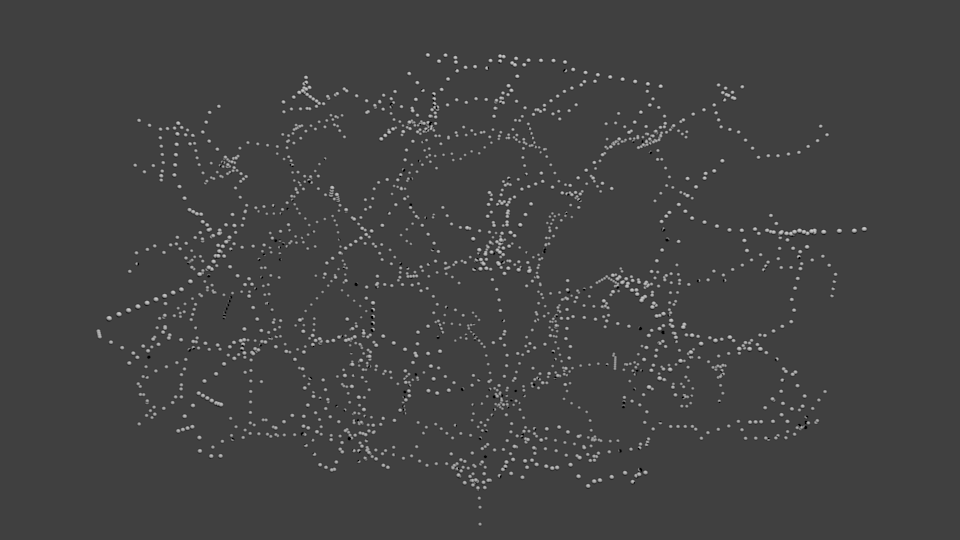
\includegraphics[scale=0.37]{nodes.png}
\caption{Distribuzione di 2180 nodi}
\centering
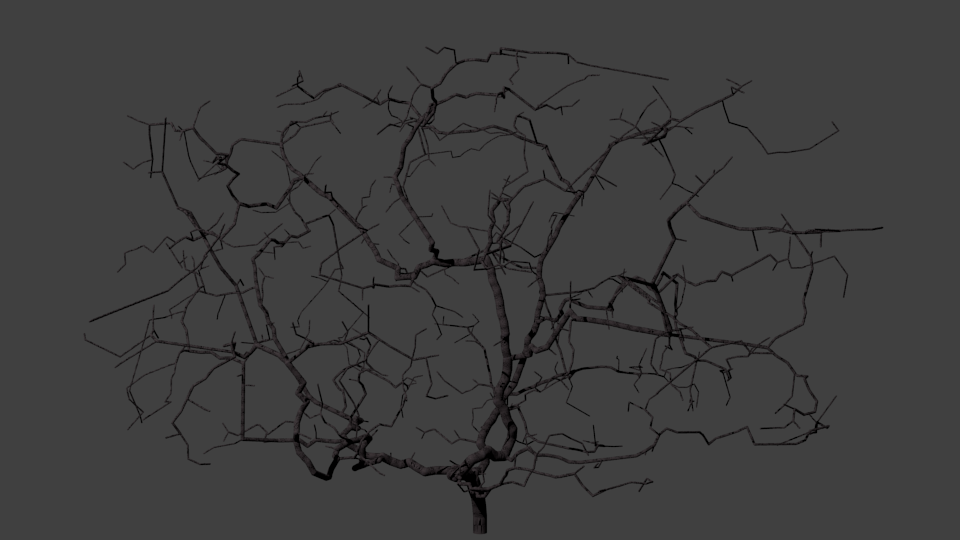
\includegraphics[scale=0.37]{tree.png}
\caption{./tree\_generator -e "envelope.obj" -p 3000 -i 20 -k 4 -d 0.06}

\end{figure}
\item \textbf{build\_branches} riceve in input i quattro vettori relativi ai nodi generati in precedenza, il raggio delle estremità dei rami, l'indice del base node e una costante $n$ compresa tra 2 e 3 (utilizzata per il calcolo del raggio dei rami). Effettua una visita DFS dei nodi dell'albero, calcolando per ogni nodo $v$ il raggio $r_v$ del ramo che lo congiunge al genitore, facendo uso del raggio dei nodi figli $F(v)$
$$r_v = \sqrt[n]{\sum_{f \in F(v)} r_f^n} $$
Per ogni nodo $v$ diverso dal base node:
\begin{itemize}
\item genera una sfera di raggio $r_v$ usando \textbf{refine\_branch} di centro (0,0,0) e poi la traslata in corrispondenza del nodo per coprire gli spazi vuoti all'intersezione dei rami
\item genera un cilindro tra v e il genitore di raggio $r_v$ di altezza $D$ 
\end{itemize}
\end{itemize}
L'implentazione dell'algoritmo è così completamente funzionante e, fornendo più envelope, ognuna di esse associata a un base node, si può generare una foresta. Il codice sorgente include alcune migliorie riguardanti la generazione di base nodes e l'introduzione di una struttura tree\_node, tuttavia, anche se sono completamente implementate, non sono integrate con le funzioni descritte in precedenza.
\begin{itemize}

\item la struct \textbf{tree\_node} è pensata per sostituire i tre vettori genitore, figli e normali. 
\item la funzione \textbf{build\_base\_nodes} genera nodi base data un envelope. Prendendo in considerazione il punto più in basso dell'envelope, genera il tronco, quindi una sequenza di base nodes finchè non vi è un attraction point che influenza uno o più di essi

\end{itemize}
{\LARGE \textbf{Immagini}}

\begin{figure}[h]
\centering
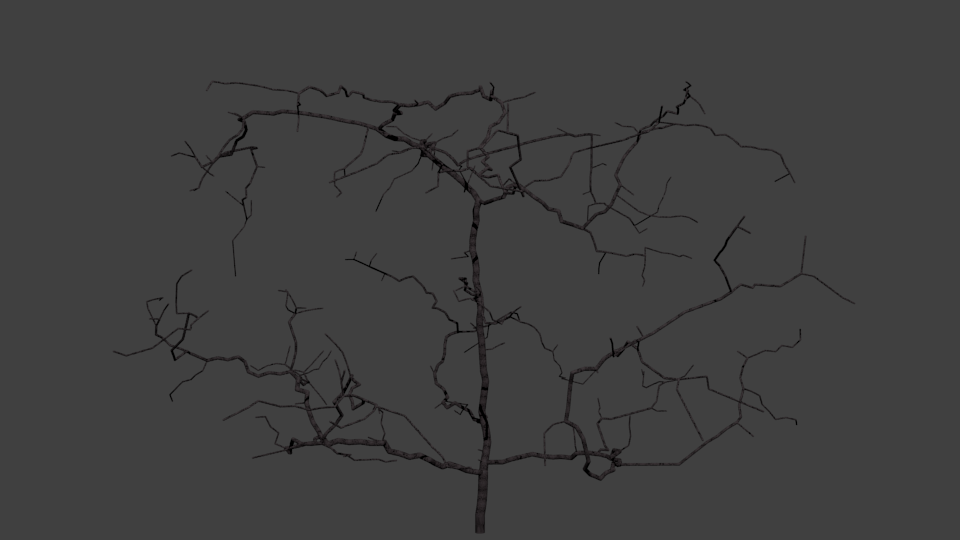
\includegraphics[scale=0.45]{figura5.png}
\caption{./tree\_generator -e "envelope.obj" -p 5000 -i 20 -k 8 -d 0.06 \textit{(kill distance elevata)}}

\end{figure}
\begin{figure}[ht!]
\centering
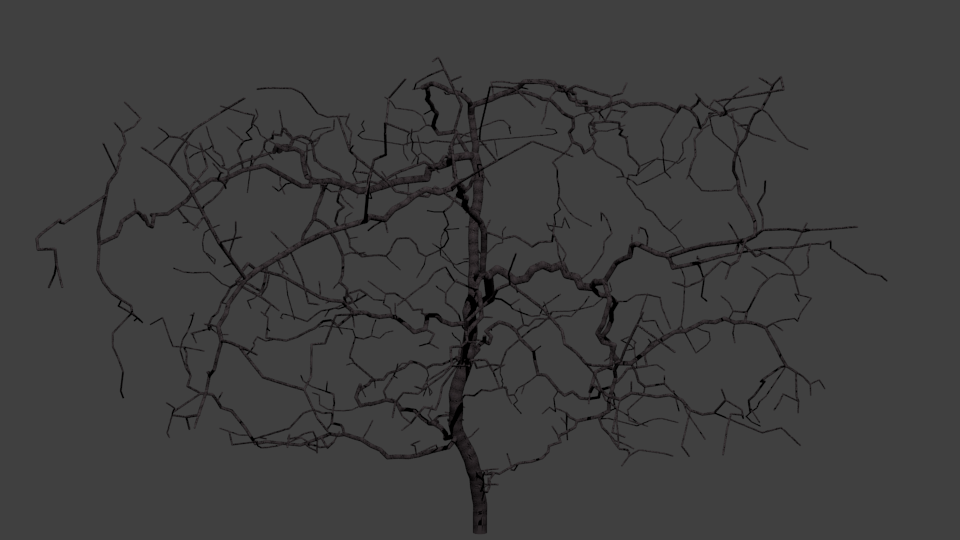
\includegraphics[scale=0.45]{figura6.png}
\caption{./tree\_generator -e "envelope.obj" -p 7000 -i 20 -k 5 -d 0.06}
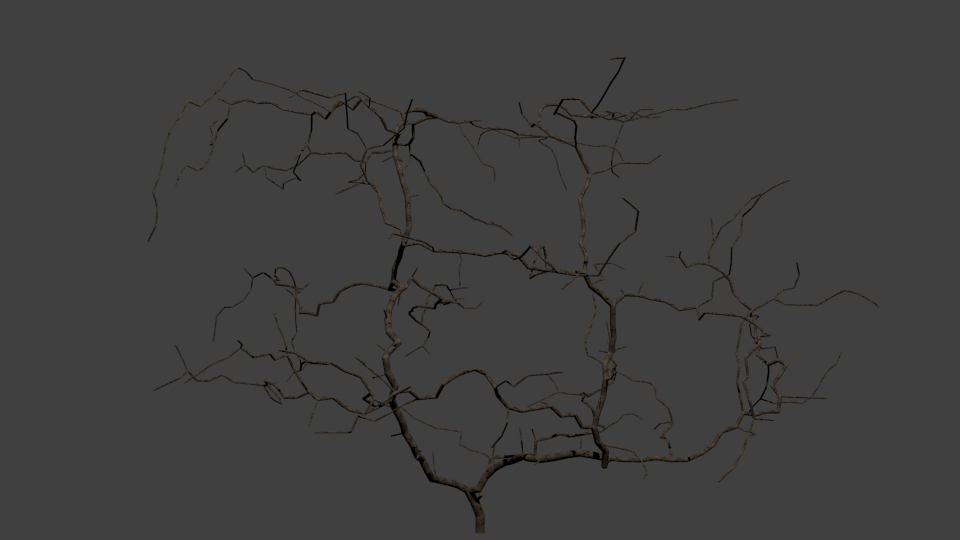
\includegraphics[scale=0.45]{figura7.png}
\caption{./tree\_generator -e "envelope.obj" -p 10000 -i 10 -k 8 -d 0.08}
\end{figure}
\begin{figure}
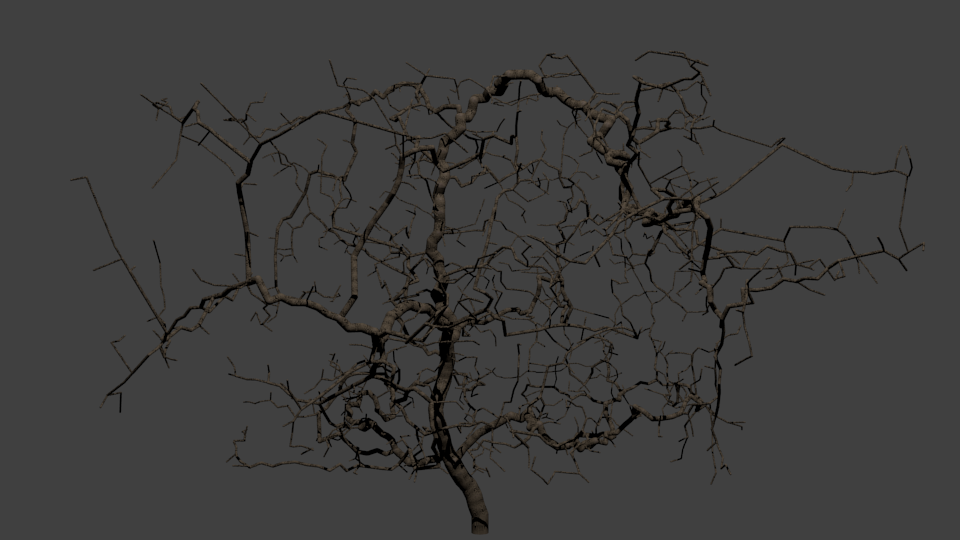
\includegraphics[scale=0.47]{figura8.png}
\caption{./tree\_generator -e "envelope.obj" -p 15000 -i 10 -k 3 -d 0.06}
\end{figure}
\end{document}